% ---------------------------------------------------------------------------
% dendritic_credit_workshop_25_core.tex — 26 core frames, no act dividers.
% Canvas assets informed composition only.  Every equation, schematic and
% data panel below is native TeX/TikZ or a vector crop from pdf_assets/.
% ---------------------------------------------------------------------------

% 1 — title
\begin{frame}[plain]
  \vspace{0.48cm}
  \begin{columns}[c,onlytextwidth]
    \begin{column}{0.58\textwidth}
      {\color{Shunt}\rule{1.15cm}{1.8pt}}\par
      \vspace{0.34cm}
      {\fontsize{25}{29}\selectfont\bfseries
       When dendritic structure helps\\[0.05cm]
       local credit assignment\par}
      \vspace{0.28cm}
      {\normalsize\color{Mute}
       Coordinates, subtree addresses, route gain, and the alignment
       boundary\par}
      \vspace{0.56cm}
      {\small Houman Safaai\enspace\textperiodcentered\enspace
       Maceo Richards\enspace\textperiodcentered\enspace
       Bernardo L. Sabatini\par}
      \vspace{0.10cm}
      {\footnotesize\color{Mute}Kempner Institute, Harvard University
       \enspace\textperiodcentered\enspace Harvard Medical School\par}
      \vspace{0.24cm}
      {\footnotesize\color{Mute}Kempner Learning Dynamics Workshop, 2026\par}
    \end{column}
    \begin{column}{0.38\textwidth}
      \centering
      \CreditTree[mode=address,K=4,scale=0.98,
        stagelabel={one neuron, multiple candidate credit routes}]
      \vspace{0.06cm}
      {\scriptsize\color{Mute}task error arrives at the soma\par}
    \end{column}
  \end{columns}
\end{frame}

% 2 — global consequence to local causes
\begin{frame}{Learning is a credit-assignment problem}
  \framesubtitle{A global consequence must ultimately guide local synaptic change.}
  \vspace{0.12cm}
  \centering
  \begin{tikzpicture}[line cap=round,>=Stealth]
    \tikzset{stage/.style={rounded corners=3pt,draw=Grid,fill=Paper,
      minimum width=2.05cm,minimum height=1.36cm,align=center,font=\scriptsize}}
    \node[stage] (beh) at (0,0) {behavior\\[-1pt]{\tiny reward or error}};
    \node[stage] (net) at (2.55,0) {network\\[-1pt]{\tiny many neurons}};
    \node[stage] (neu) at (5.10,0) {neuron\\[-1pt]{\tiny many branches}};
    \node[stage] (bra) at (7.65,0) {subtree\\[-1pt]{\tiny many synapses}};
    \node[stage] (syn) at (10.20,0) {synapse\\[-1pt]{\tiny one parameter}};
    \foreach \a/\b in {beh/net,net/neu,neu/bra,bra/syn}
      \draw[Mute,-{Stealth[length=4.5pt]},line width=0.9pt] (\a) -- (\b);
    \node[circle,fill=BP!14,draw=BP,line width=0.7pt,minimum size=9pt]
      at (0,0.34) {};
    \foreach \y in {-0.34,0,0.34}
      \node[circle,fill=white,draw=Add,line width=0.6pt,minimum size=5pt]
        at (2.30,\y) {};
    \draw[Dend,line width=1.0pt] (5.10,-0.30) -- (5.10,0.20)
      -- (4.78,0.55) (5.10,0.20) -- (5.42,0.55);
    \filldraw[fill=Soma,draw=Ink!30] (5.10,-0.38) circle (0.10);
    \draw[Dend,line width=0.9pt] (7.65,-0.32) -- (7.65,0.18)
      -- (7.32,0.52) (7.65,0.18) -- (7.98,0.52);
    \fill[Exc] (10.20,0.18) circle (0.08);
    \draw[Mute,line width=0.8pt] (10.20,0.10) -- (10.20,-0.36);
    \node[font=\tiny,text=BP,anchor=north] at (0,-0.86) {one loss};
    \node[font=\tiny,text=Mute,anchor=north] at (5.10,-0.86) {which neuron?};
    \node[font=\tiny,text=Mute,anchor=north] at (7.65,-0.86) {which branch?};
    \node[font=\tiny,text=Mute,anchor=north] at (10.20,-0.86) {which weight?};
  \end{tikzpicture}
  \vspace{0.28cm}
  \heroeq[the assignment]{%
    \text{which parameter changes?}\quad
    \text{which direction?}\quad
    \text{how much?}}
  \vfill
  \takeaway{The loss is global, but every update must be local and correctly addressed.}
  \vspace{0.04cm}
\end{frame}

% 3 — exact BP reference
\begin{frame}{Backpropagation provides exact parameter credit}
  \framesubtitle{It is the optimization reference against which local rules are compared.}
  \begin{columns}[c,onlytextwidth]
    \begin{column}{0.39\textwidth}
      \centering
      \begin{tikzpicture}[line cap=round]
        \foreach \x/\n/\c in {0/a/Add,1.35/b/Shunt,2.70/c/Violet,4.05/d/BP}{
          \foreach \y/\k in {0/1,0.66/2,1.32/3}{
            \node[circle,draw=\c,fill=white,line width=0.7pt,
              inner sep=0pt,minimum size=7pt] (\n\k) at (\x,\y) {};}}
        \foreach \i in {1,2,3}\foreach \j in {1,2,3}{
          \draw[Grid,line width=0.45pt] (a\i)--(b\j);
          \draw[Grid,line width=0.45pt] (b\i)--(c\j);
          \draw[Grid,line width=0.45pt] (c\i)--(d\j);}
        \node[rounded corners=2pt,draw=BP,fill=BP!7,font=\scriptsize,
          inner sep=3pt] (loss) at (5.05,0.66) {$\mathcal L$};
        \draw[Mute,line width=0.7pt] (d2)--(loss);
        \draw[BP,-{Stealth[length=4pt]},line width=1.0pt]
          (4.72,-0.30) -- (0.18,-0.30);
        \node[font=\tiny,text=BP,anchor=north] at (2.45,-0.43)
          {coordinated reverse pass};
      \end{tikzpicture}
    \end{column}
    \begin{column}{0.57\textwidth}
      \heroeq[exact update]{%
        \Delta W^{\ell}_{ji}=-\eta\,
        \term[Shunt]{h^{\ell-1}_{i}}{presynaptic activity}\,
        \term[Add]{\delta^{\ell}_{j}}{parameter-specific error}}
      \vspace{0.12cm}
      \heroeq[reverse recursion]{%
        \bm\delta^{\ell}=
        (W^{\ell+1})^{\mathsf T}\bm\delta^{\ell+1}
        \odot f'(\bm a^{\ell})}
      \vspace{0.10cm}
      {\footnotesize\color{Mute}Every weight receives a signed magnitude and
       an exact destination.\par}
    \end{column}
  \end{columns}
  \vfill
  \takeaway{Backpropagation answers credit assignment exactly, one parameter at a time.}
  \vspace{0.04cm}
\end{frame}

% 4 — biological implementation gap
\begin{frame}{Literal backpropagation is not a neuronal mechanism}
  \framesubtitle{The question is which information a synapse can actually access.}
  \vspace{0.08cm}
  \begin{columns}[T,onlytextwidth]
    \begin{column}{0.64\textwidth}
      \begin{columns}[T,onlytextwidth]
        \begin{column}{0.48\textwidth}
          \claimbox{\deftag{weight transport}\par
            {\footnotesize reuse exact downstream weights in reverse\par}}
          \vspace{0.15cm}
          \claimbox{\deftag{global coordination}\par
            {\footnotesize ordered Jacobian products across layers\par}}
        \end{column}
        \begin{column}{0.48\textwidth}
          \claimbox{\deftag{nonlocal state}\par
            {\footnotesize downstream derivatives at the same learning event\par}}
          \vspace{0.15cm}
          \claimbox{\deftag{parameter indexing}\par
            {\footnotesize a distinct error coordinate for every destination\par}}
        \end{column}
      \end{columns}
      \vspace{0.22cm}
      {\footnotesize Biological theories replace, approximate, infer, or
       physically instantiate different pieces of this reverse computation.\par}
    \end{column}
    \begin{column}{0.32\textwidth}
      \centering
      \CreditTree[mode=eligibility,scale=0.86,
        stagelabel={what a synapse can measure locally}]
    \end{column}
  \end{columns}
  \vfill
  \takeaway{A plausible rule must say what replaces the exact synaptic error.}
  \vspace{0.04cm}
\end{frame}

% 5 — state of the art
\begin{frame}{Local-learning theories differ in what replaces the exact error}
  \framesubtitle{Different mechanisms often resolve credit only to the level of a neuron.}
  \vspace{0.04cm}
  \begin{columns}[T,onlytextwidth]
    \begin{column}{0.235\textwidth}
      \claimbox{\deftag{modulatory scalar}\par
        \vspace{0.06cm}{\small$\Delta w_i\propto e_i m$\par}
        \vspace{0.10cm}{\scriptsize\color{Mute}three-factor rules\par}}
    \end{column}
    \begin{column}{0.235\textwidth}
      \claimbox{\deftag{feedback alignment}\par
        \vspace{0.06cm}{\small$\widehat{\bm\delta}=B\bm\delta^{\rm out}$\par}
        \vspace{0.10cm}{\scriptsize\color{Mute}fixed/random routes\par}}
    \end{column}
    \begin{column}{0.235\textwidth}
      \claimbox{\deftag{state inference}\par
        \vspace{0.06cm}{\small$\widehat\delta\sim s^{+}-s^{-}$\par}
        \vspace{0.10cm}{\scriptsize\color{Mute}predictive/equilibrium\par}}
    \end{column}
    \begin{column}{0.235\textwidth}
      \claimbox{\deftag{error compartments}\par
        \vspace{0.06cm}{\small$\widehat\delta_u$ beside $a_u$\par}
        \vspace{0.10cm}{\scriptsize\color{Mute}apical/basal models\par}}
    \end{column}
  \end{columns}
  \vspace{0.32cm}
  \centering
  \begin{tikzpicture}[line cap=round]
    \draw[Amber,line width=2.4pt] (0,0)--(1.45,0);
    \draw[Add,line width=2.4pt] (2.10,0)--(3.55,0);
    \draw[Violet,line width=2.4pt] (4.20,0)--(5.65,0);
    \draw[Dend,line width=2.4pt] (6.30,0)--(7.75,0);
    \node[font=\scriptsize,text=Amber,anchor=north] at (0.72,-0.18) {one scalar};
    \node[font=\scriptsize,text=Add,anchor=north] at (2.82,-0.18) {one coordinate};
    \node[font=\scriptsize,text=Violet,anchor=north] at (4.92,-0.18) {inferred coordinate};
    \node[font=\scriptsize,text=Dend,anchor=north] at (7.02,-0.18) {few compartments};
  \end{tikzpicture}
  \srcnote{Fr\'emaux \& Gerstner 2016; Lillicrap et al. 2016; Scellier \& Bengio 2017;
    Whittington \& Bogacz 2017; Guerguiev et al. 2017; Sacramento et al. 2018;
    Payeur et al. 2021.}
  \vfill
  \takeaway{The unresolved spatial step begins after a neuron-level teaching coordinate arrives.}
  \vspace{0.04cm}
\end{frame}

% 6 — point-neuron bottleneck
\begin{frame}{Point-neuron learning stops at one neuronal coordinate}
  \begin{columns}[T,onlytextwidth]
    \begin{column}{0.59\textwidth}
      {\scriptsize\color{Mute}point neuron:
       $s_u=\sum_iw_ix_i$, $V_u=f(s_u)$\par}
      \heroeq[point-neuron rule]{%
        \frac{\partial\mathcal L}{\partial w_i}
        =\term[Shunt]{x_if'(s_u)}{synapse-local eligibility}\,
         \term[Add]{\delta_u}{one shared coordinate}}
      \vspace{0.14cm}
      {\footnotesize Different inputs keep weights and activities distinct,
       but no variable can assign different teaching coordinates to two
       subtrees of the same neuron.\par}
      \vspace{0.12cm}
      {\footnotesize\color{Mute}The bottleneck is feedback bandwidth, not a
       collapse of all neurons into one.\par}
    \end{column}
    \begin{column}{0.37\textwidth}
      \centering
      \CreditTree[mode=coordinate,scale=1.06,
        stagelabel={one coordinate reaches the soma}]
    \end{column}
  \end{columns}
  \vfill
  \takeaway{Point neurons distinguish synapses through eligibility, but cannot explicitly address locations inside the arbor.}
  \vspace{0.04cm}
\end{frame}

% 7 — preview of dendritic additions
\begin{frame}{A dendritic tree adds state, addresses, and route gain}
  \heroeq*[preview]{%
    \frac{\partial\mathcal L}{\partial g_i}
    =\term[Shunt]{e_i}{local state}\,
     \term[Add]{\delta_{0,u}}{neuron coordinate}\,
     \term[Dend]{\widetilde\alpha_{n(i)}}{transport/path gain}}
  \vspace{0.14cm}
  \centering
  \resizebox{0.94\textwidth}{!}{%
    \TreeStrip{\CreditTree[mode=eligibility,scale=0.57,stagelabel={local state}]}%
              {\CreditTree[mode=coordinate,scale=0.57,stagelabel={which neuron?}]}%
              {\CreditTree[mode=address,K=4,scale=0.57,stagelabel={where in the tree?}]}%
              {\CreditTree[mode=gain,scale=0.57,stagelabel={how strongly?}]}\relax}\par
  \vfill
  \raggedright
  \takeaway{The tree adds spatial structure after the neuronal coordinate arrives; whether it helps is an alignment question.}
  \vspace{0.04cm}
\end{frame}
% 8 — forward conductance tree and shunting
\begin{frame}{A dendritic neuron is a conductance tree}
  \framesubtitle{The steady state is a conductance-weighted quotient at every compartment.}
  \begin{columns}[T,onlytextwidth]
    \begin{column}{0.63\textwidth}
      \heroeq[steady-state compartment]{%
        V_n=R_n^{\mathrm{tot}}
        \Bigl(\sum_{i\in\mathcal S_n}g_ix_iE_i
        +\sum_{c\in\mathcal C_n}g^{\mathrm{den}}_{c\to n}a_c
        +g_n^{\mathrm{sh}}E_I+g_n^LE_L\Bigr)}
      \vspace{0.05cm}
      {\scriptsize\color{Mute}
       $R_n^{\mathrm{tot}}=(g_n^{\mathrm{tot}})^{-1}$,
       $\ g_n^{\mathrm{tot}}=g_n^L+\sum_i g_ix_i
          +\sum_c g^{\mathrm{den}}_{c\to n}+g_n^{\mathrm{sh}}$\par}
      \vspace{0.16cm}
      \claimbox{\deftag{shunting}\par
        {\footnotesize A local inhibitory conductance raises the denominator,
         alters the compartment state, and edits the transport operator.\par}}
    \end{column}
    \begin{column}{0.33\textwidth}
      \centering
      \CreditTree[mode=forward,scale=0.70,
        stagelabel={signals integrate from leaves to soma}]
      \vspace{0.02cm}
      \CreditTree[mode=shunt,shunted=true,scale=0.42,
        stagelabel={a local shunt edits descendant paths}]
    \end{column}
  \end{columns}
  \vfill
  \takeaway{Shunting is central because it changes both the forward state and the backward sensitivity operator.}
  \vspace{0.04cm}
\end{frame}

% 9 — exact local eligibility
\begin{frame}{The conductance quotient yields an exact local eligibility}
  \begin{columns}[T,onlytextwidth]
    \begin{column}{0.63\textwidth}
      \heroeq[quotient rule]{%
        \frac{\partial V_n}{\partial g_i}
        =\term[Shunt]{x_i}{presynaptic activity}\,
         \term[Shunt]{R_n^{\mathrm{tot}}}{input resistance}\,
         \term[Shunt]{(E_i-V_n)}{driving force}
        \equiv e_i}
      \vspace{0.16cm}
      {\footnotesize The same synapse has access to all three factors: its
       presynaptic activity, local voltage, and local conductance state.\par}
      \vspace{0.12cm}
      \claimbox{\footnotesize In an additive-current model the denominator
        does not depend on the synaptic weight; the driving-force term is
        absent.\par}
    \end{column}
    \begin{column}{0.33\textwidth}
      \centering
      \CreditTree[mode=eligibility,scale=0.92,
        stagelabel={all factors are available at the synapse}]
    \end{column}
  \end{columns}
  \vfill
  \takeaway{Conductance normalization preserves locality and creates the exact driving-force factor.}
  \vspace{0.04cm}
\end{frame}

% 10 — transported error field
\begin{frame}{Each compartment receives a transported error field}
  \framesubtitle{On a tree, every compartment has one unique route to the soma.}
  \begin{columns}[T,onlytextwidth]
    \begin{column}{0.58\textwidth}
      \heroeq[compartment error]{%
        \delta_n\equiv\frac{\partial\mathcal L}{\partial V_n}
        =\delta_{0,u}\,\widetilde\alpha_n}
      \vspace{0.12cm}
      \heroeq[path gain]{%
        \widetilde\alpha_n=
        \prod_{(j\to k)\in\operatorname{path}(n\to0)}
        f'_j(V_j)\,R_k^{\mathrm{tot}}\,g^{\mathrm{den}}_{j\to k}}
      \vspace{0.08cm}
      {\footnotesize\color{Mute}The route gain is state-dependent and
       multiplicative; a shunt changes factors on descendant paths.\par}
    \end{column}
    \begin{column}{0.38\textwidth}
      \centering
      \CreditTree[mode=transport,scale=1.02,
        stagelabel={the somatic error transported to one site}]
    \end{column}
  \end{columns}
  \vfill
  \takeaway{The teaching signal at a synapse is a somatic coordinate multiplied by transport along its branch path.}
  \vspace{0.04cm}
\end{frame}

% 11 — exact factorization
\begin{frame}{Exact dendritic credit factorizes at every synapse}
  \framesubtitle{The factorization separates what is local from what must be routed.}
  \vspace{0.10cm}
  \heroeq*[theorem]{%
    \frac{\partial\mathcal L}{\partial g_i}
    =\term[Shunt]{x_iR_{n(i)}^{\mathrm{tot}}(E_i-V_{n(i)})}{local eligibility $e_i$}\,
     \term[Add]{\delta_{0,u}\widetilde\alpha_{n(i)}}{transported error $\delta_{n(i)}$}}
  \vspace{0.24cm}
  \begin{columns}[c,onlytextwidth]
    \begin{column}{0.31\textwidth}
      \centering
      \CreditTree[mode=eligibility,scale=0.53,stagelabel={computed locally}]
    \end{column}
    \begin{column}{0.08\textwidth}
      \centering{\Large$\times$}
    \end{column}
    \begin{column}{0.31\textwidth}
      \centering
      \CreditTree[mode=transport,scale=0.53,stagelabel={delivered along the tree}]
    \end{column}
    \begin{column}{0.24\textwidth}
      {\footnotesize\color{Mute}Exact reconstruction matched autodiff across
       100 diagnostic runs; relative discrepancies were at numerical
       precision.\par}
    \end{column}
  \end{columns}
  \vfill
  \takeaway{Local learning becomes a question of how faithfully biology approximates the transported field.}
  \vspace{0.04cm}
\end{frame}

% 12 — hierarchy of teaching fields
\begin{frame}{Credit fields form a hierarchy of spatial resolution}
  \framesubtitle{Each rung preserves more destination information and costs more feedback bandwidth.}
  \centering
  \vspace{0.18cm}
  \resizebox{0.94\textwidth}{!}{%
    \TreeStrip{\CreditTree[mode=scalar,scale=0.59,
          stagelabel={\shortstack{global scalar\\[-1pt]{\color{Amber}\bfseries which example?}}}]}%
      {\CreditTree[mode=coordinate,scale=0.59,
          stagelabel={\shortstack{neuron coordinate\\[-1pt]{\color{Add}\bfseries which neuron?}}}]}%
      {\CreditTree[mode=address,K=4,scale=0.59,
          stagelabel={\shortstack{subtree addresses\\[-1pt]{\color{Dend}\bfseries where in the tree?}}}]}%
      {\CreditTree[mode=transport,scale=0.59,
          stagelabel={\shortstack{exact compartment field\\[-1pt]{\color{Violet}\bfseries which compartment?}}}]}\relax}\par
  \vspace{0.22cm}
  \begin{tikzpicture}[line cap=round]
    \draw[Amber,line width=2.6pt] (0,0)--(2.1,0);
    \draw[Add,line width=2.6pt] (2.1,0)--(4.2,0);
    \draw[Dend,line width=2.6pt] (4.2,0)--(6.3,0);
    \draw[Violet,line width=2.6pt] (6.3,0)--(8.4,0);
    \node[font=\tiny,text=Mute,anchor=north] at (0,-0.16) {low bandwidth};
    \node[font=\tiny,text=Mute,anchor=north] at (8.4,-0.16) {high bandwidth};
  \end{tikzpicture}\par
  \vspace{0.04cm}
  {\scriptsize\color{Mute}Route gain rescales an available coordinate; it does
   not add feedback bandwidth.\par}
  \vfill
  \raggedright
  \takeaway{Neuron identity and within-tree address are distinct credit-assignment problems.}
  \vspace{0.04cm}
\end{frame}

% 13 — stochastic operator utility
\begin{frame}{A credit operator predicts when restricted routes help}
  {\scriptsize\color{Mute}teaching field
   $\widehat{\bm g}=\bm g+\bm\xi$, update
   $\bm w^{+}=\bm w-\eta M\widehat{\bm g}$, noise covariance $\Sigma$\par}
  \heroeq[descent bound]{%
    \E\mathcal L(\bm w^{+})\leq\mathcal L(\bm w)
      -\eta\,\term[Shunt]{\bm g^{\mathsf T}M\bm g}{retained task signal}
      +\frac{L\eta^2}{2}\left(
        \term[Amber]{\lVert M\bm g\rVert_2^2}{curvature cost}
        +\term[BP]{\tr(M\Sigma M^{\mathsf T})}{admitted noise}\right)}
  \vspace{0.12cm}
  \heroeq[optimized one-step utility]{%
    U(M)=\frac{[\bm g^{\mathsf T}M\bm g]^2}
      {2L\{\lVert M\bm g\rVert_2^2+\tr(M\Sigma M^{\mathsf T})\}},
    \qquad \bm g^{\mathsf T}M\bm g>0}
  \vspace{0.04cm}
  {\scriptsize Positivity is feedback alignment; the expression is exact for
   the matched quadratic and otherwise orders guarantees.\par}
  \vfill
  \takeaway{A restricted route helps only if what it preserves outweighs what it discards or admits as noise.}
  \vspace{0.04cm}
\end{frame}

% 14 — theory-guided phase prediction
\begin{frame}{Alignment $\times$ bandwidth defines the phase boundary}
  \framesubtitle{This is the theory-guided prediction; the populated evidence map returns near the end.}
  \begin{columns}[T,onlytextwidth]
    \begin{column}{0.48\textwidth}
      \heroeq[unit-step identity-quadratic crossover]{%
        \term[BP]{\tr[(I-P)\Sigma]}{rejected noise}
        >\term[Add]{\lVert(I-P)\bm g\rVert_2^2}{discarded task signal}}
      \vspace{0.14cm}
      {\footnotesize Too few routes discard signal; too many routes admit
       fine-scale noise. An interior bandwidth can therefore be optimal.\par}
      \vspace{0.16cm}
      \begin{columns}[T,onlytextwidth]
        \begin{column}{0.47\textwidth}
          \headline[Shunt]{$\rho_s=0.937$}{predicted vs. observed one-step progress}
        \end{column}
        \begin{column}{0.47\textwidth}
          \headline[Violet]{$\rho_s=0.916$}{predicted utility vs. final held-out accuracy}
        \end{column}
      \end{columns}
    \end{column}
    \begin{column}{0.48\textwidth}
      \centering
      \begin{tikzpicture}[line cap=round]
        \fill[BP!8] (0,0) rectangle (5.2,3.55);
        \fill[Amber!18] (0.55,0.42) .. controls (1.9,1.0) and (2.9,2.2) ..
          (3.2,3.55) -- (5.2,3.55) -- (5.2,0) -- (0,0) -- cycle;
        \fill[ShuntPale] (2.0,0.62) .. controls (2.85,1.5) and (3.15,2.6) ..
          (3.45,3.55) -- (5.2,3.55) -- (5.2,0.72) -- cycle;
        \draw[white,line width=1.2pt,dash pattern=on 4pt off 3pt]
          (0.55,0.42) .. controls (1.9,1.0) and (2.9,2.2) .. (3.2,3.55);
        \draw[white,line width=1.2pt,dash pattern=on 4pt off 3pt]
          (2.0,0.62) .. controls (2.85,1.5) and (3.15,2.6) .. (3.45,3.55);
        \draw[Ink,-{Stealth[length=4pt]},line width=0.7pt] (0,0)--(5.45,0);
        \draw[Ink,-{Stealth[length=4pt]},line width=0.7pt] (0,0)--(0,3.82);
        \node[font=\scriptsize\bfseries,text=Ink,anchor=north] at (2.65,-0.34)
          {task–route alignment};
        \node[font=\scriptsize\bfseries,text=Ink,rotate=90,anchor=south]
          at (-0.48,1.78) {route bandwidth};
        \node[font=\scriptsize\bfseries,text=BP] at (0.95,2.83) {signal lost};
        \node[font=\scriptsize\bfseries,text=Amber!72!Ink] at (2.55,1.55)
          {matched regime};
        \node[font=\scriptsize\bfseries,text=Shunt!72!Ink] at (4.15,2.65)
          {routes help};
      \end{tikzpicture}
      \vspace{0.06cm}
      {\scriptsize\color{Mute}schematic prediction, not a measured phase diagram\par}
    \end{column}
  \end{columns}
  \vfill
  \takeaway{The theory predicts both the wins and the nulls before anatomy enters the analysis.}
  \vspace{0.04cm}
\end{frame}
% 15 — identity and ownership
\begin{frame}{Neuron identity closes most of the ordinary classification gap}
  \framesubtitle{Bandwidth selects the neuron; ownership supplies a smaller map-specific refinement.}
  \begin{columns}[T,onlytextwidth]
    \begin{column}{0.52\textwidth}
      \centering
      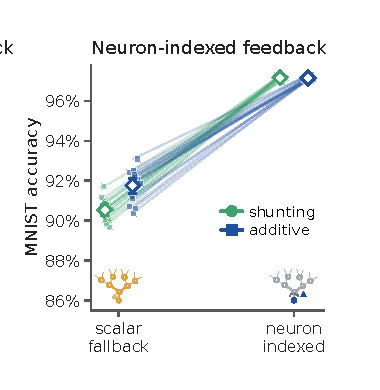
\includegraphics[width=\linewidth,height=3.45cm,keepaspectratio]{pdf_assets/identity_panel_b.pdf}\par
      \raggedright
      \headline[Add]{$7.8$--$11.2$ pp}{strict scalar $\rightarrow$
        neuron-specific feedback on MNIST}
    \end{column}
    \begin{column}{0.44\textwidth}
      \centering
      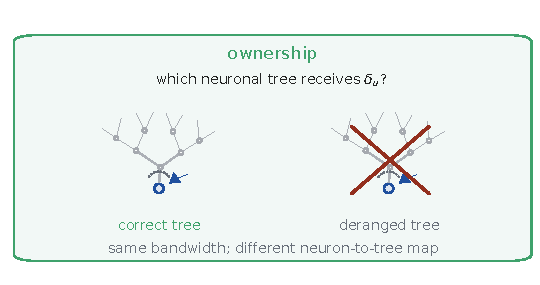
\includegraphics[width=\linewidth,height=1.50cm,keepaspectratio]{pdf_assets/ownership_schematic.pdf}\par
      \vspace{0.03cm}
      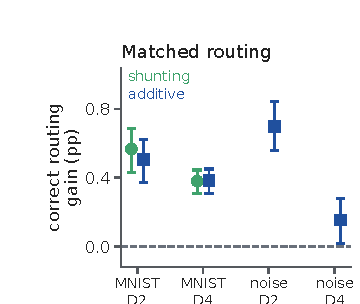
\includegraphics[width=0.82\linewidth,height=1.80cm,keepaspectratio]{pdf_assets/ownership_margin.pdf}\par
      {\scriptsize\color{Mute}same coordinates and bandwidth; only the
       neuron-to-tree assignment changes\par}
      \raggedright
      \vspace{0.06cm}
      {\large\bfseries\color{Add}$+0.15$ to $+0.70$ pp\par}
      {\scriptsize\color{Mute}correct ownership, favored in 58/60 paired comparisons\par}
    \end{column}
  \end{columns}
  \vfill
  \takeaway{The dominant bottleneck is neuron identity; routing inside the chosen neuron is a second, smaller problem on these tasks.}
  \vspace{0.04cm}
\end{frame}

% 16 — credit-conflict task and analytic boundary
\begin{frame}{Credit conflict creates demand for a branch address}
  \framesubtitle{Every branch gets a nonzero view; context selects the task-relevant one downstream.}
  \begin{columns}[T,onlytextwidth]
    \begin{column}{0.53\textwidth}
      \centering
      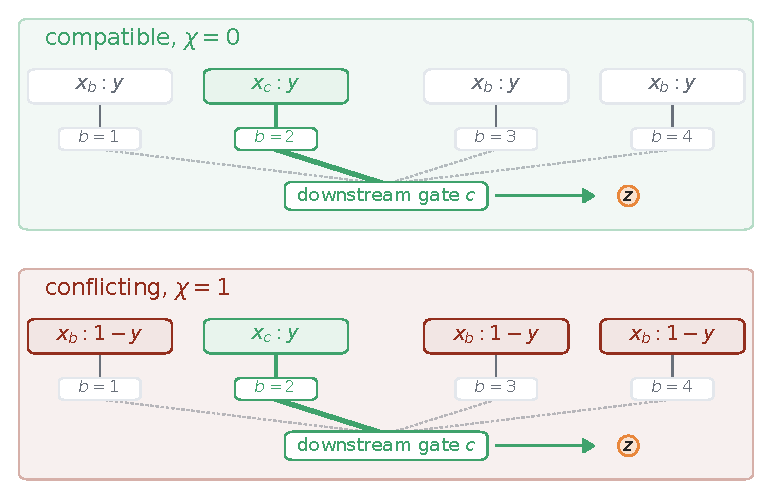
\includegraphics[width=\linewidth,height=4.52cm,keepaspectratio]
        {pdf_assets/path_necessity_task.pdf}\par
    \end{column}
    \begin{column}{0.43\textwidth}
      \deftag{conflict dose}\par
      {\footnotesize With probability $\chi$, every nonselected view carries the
       opposite class; otherwise it agrees.  The selector lies downstream of
       branch-local eligibility, so all $B$ local traces remain nonzero.\par}
      \vspace{0.07cm}
      \begin{columns}[T,totalwidth=\linewidth]
        \begin{column}{0.48\linewidth}
          {\scriptsize\color{Shunt}\bfseries correct path\par}
          {\small\color{Shunt}$\delta_b=\delta\mathbf 1[b=c]$\par}
        \end{column}
        \begin{column}{0.48\linewidth}
          {\scriptsize\color{Amber}\bfseries neuron shared\par}
          {\small\color{Amber}$\widetilde\delta_b=\delta/B$\par}
        \end{column}
      \end{columns}
      \vspace{0.08cm}
      \claimbox{\deftag{analytic boundary}\par
        \vspace{0.05cm}
        {\small
        \[
          C_{\chi}=(1-2\chi)\bm 1\bm 1^{\mathsf T}+2\chi I_B,
        \]
        \vspace{-0.22cm}
        \[
          \lambda_{\parallel}=B-2\chi(B-1),\qquad
          \chi_c(B)=\frac{B}{2(B-1)}.
        \]}}
    \end{column}
  \end{columns}
  \vfill
  \takeaway{This isolates a need for branch-selective information, not a dendrite-exclusive material implementation.}
  \vspace{0.04cm}
\end{frame}

% 17 — confirmatory path-necessity result
\begin{frame}{The path benefit appears at the predicted conflict boundary}
  \framesubtitle{Twenty confirmatory seeds; correct path, analytic backpropagation, and gated-point emulation coincide.}
  \begin{columns}[T,onlytextwidth]
    \begin{column}{0.73\textwidth}
      \centering
      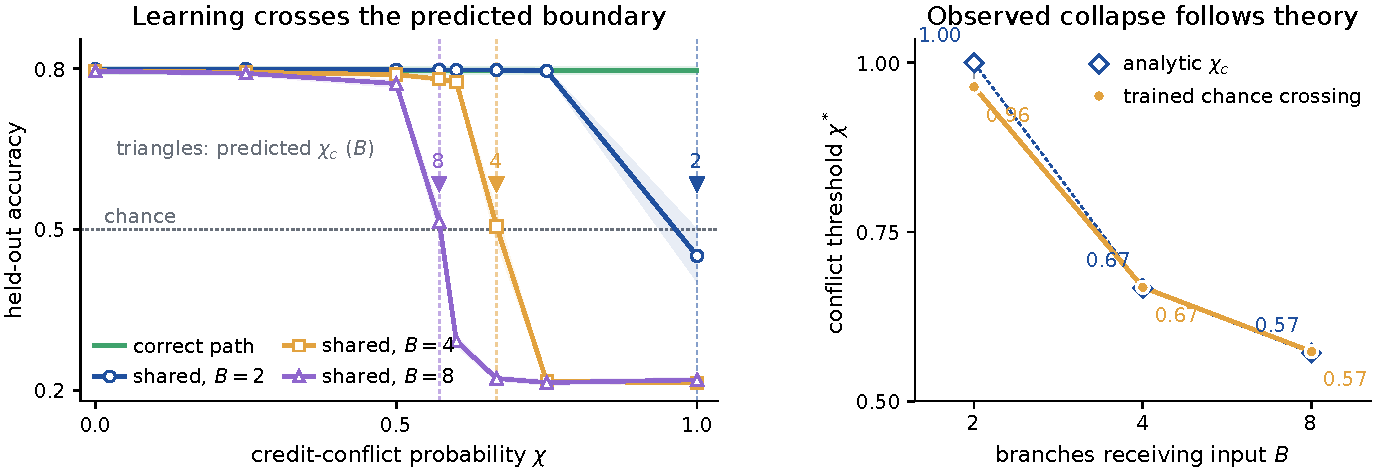
\includegraphics[width=\linewidth,height=4.72cm,keepaspectratio]
        {pdf_assets/path_necessity_results.pdf}\par
    \end{column}
    \begin{column}{0.23\textwidth}
      \vspace{0.03cm}
      \deftag{no conflict}\par
      {\footnotesize $\chi=0$: mean correct-minus-shared difference
       $\leq0.16$ percentage points.\par}
      \vspace{0.11cm}
      \headline[Shunt]{$+58.2$ pp}{correct path minus shared credit at
        $B=4$, $\chi=1$}
      \vspace{0.08cm}
      \deftag{ordered transition}\par
      {\large\bfseries $\chi^*_{8}<\chi^*_{4}<\chi^*_{2}$\par}
      {\scriptsize\color{Mute}utility and trained accuracy; 20/20 seeds\par}
    \end{column}
  \end{columns}
  \vfill
  \takeaway{Branch-selective credit pays only when nonselected branches carry conflicting evidence.}
  \vspace{0.04cm}
\end{frame}

% 18 — ancestry budget sweep
\begin{frame}{Ancestry routes help only at intermediate bandwidth}
  \framesubtitle{The benefit is consistent with an interior-bandwidth regime and disappears at full rank.}
  \begin{columns}[T,onlytextwidth]
    \begin{column}{0.40\textwidth}
      \centering
      \CreditTree[mode=address,K=4,scale=0.91,
        stagelabel={four nested ancestry routes}]
      \raggedright
      \headline[Dend]{$+1.27$ pp at $K=4$}{versus the best rank-matched
        non-anatomical route}
    \end{column}
    \begin{column}{0.56\textwidth}
      \centering
      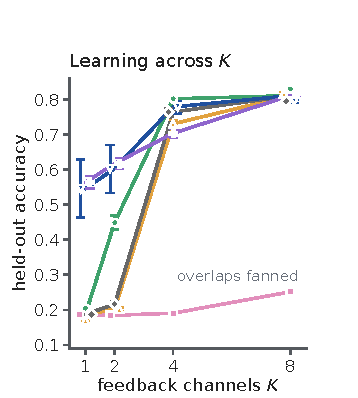
\includegraphics[width=\linewidth,height=5.20cm,keepaspectratio]{pdf_assets/subtree_k_sweep.pdf}\par
    \end{column}
  \end{columns}
  \vfill
  \takeaway{Anatomical ancestry is conditionally useful, not universally optimal.}
  \vspace{0.04cm}
\end{frame}

% 19 — physical depth
\begin{frame}{Physical depth helps only for task-matched serial computation}
  \framesubtitle{Depth is an inductive bias, not a free source of accuracy.}
  \begin{columns}[T,onlytextwidth]
    \begin{column}{0.48\textwidth}
      \centering
      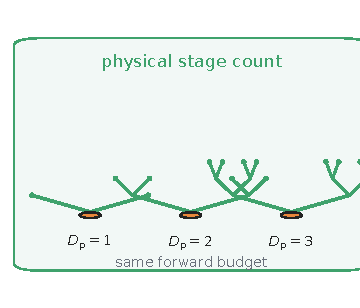
\includegraphics[width=\linewidth,height=2.10cm,keepaspectratio]{pdf_assets/physical_stage_schematic.pdf}\par
      \vspace{0.07cm}
      \eqstrip{V_n=\frac{E_n+C_n}{1+E_n+I_n+G_n+\epsilon}}
      \raggedright
      \headline[Shunt]{$+31$ pp}{aligned D3 minus D1 on a constructed
        multiplicative hierarchy, with branch units and parameters matched}
    \end{column}
    \begin{column}{0.48\textwidth}
      \centering
      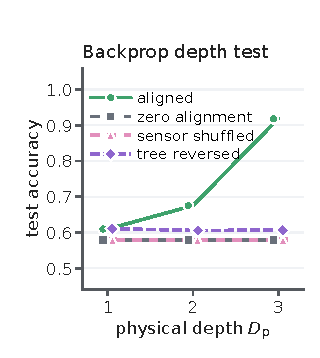
\includegraphics[width=\linewidth,height=3.85cm,keepaspectratio]{pdf_assets/physical_depth_headline.pdf}\par
      \vspace{0.06cm}
      {\scriptsize Independent sensors, shuffled sensors, and reversed order
       remain flat; at fixed budgets, depth per se reduced accuracy in 40/40
       seeds.\par}
    \end{column}
  \end{columns}
  \vfill
  \takeaway{Serial dendrites help only when the hierarchy of computation matches the hierarchy of the task.}
  \vspace{0.04cm}
\end{frame}

% 20 — reconstructed arbors
\begin{frame}{Reconstructed arbors provide sparse candidate routes}
  \framesubtitle{Morphology supplies capacity; it does not establish that endogenous learning uses it.}
  \begin{columns}[T,onlytextwidth]
    \begin{column}{0.40\textwidth}
      \centering
      \CreditTree[mode=address,K=8,scale=0.82,
        stagelabel={an ancestry dictionary with eight channels}]
      \vspace{0.05cm}
      \begin{columns}[T,totalwidth=\linewidth]
        \begin{column}{0.47\linewidth}
          {\fontsize{17}{19}\selectfont\bfseries\color{Shunt}$85\%$\par}
          {\fontsize{7}{8.4}\selectfont\color{Mute}dense-field capture at
            approximately 7\% of dense wiring\par}
        \end{column}
        \begin{column}{0.47\linewidth}
          {\fontsize{17}{19}\selectfont\bfseries\color{Violet}$2.7\times$\par}
          {\fontsize{7}{8.4}\selectfont\color{Mute}capture per connection
            beyond a density-matched shuffle\par}
        \end{column}
      \end{columns}
    \end{column}
    \begin{column}{0.56\textwidth}
      \centering
      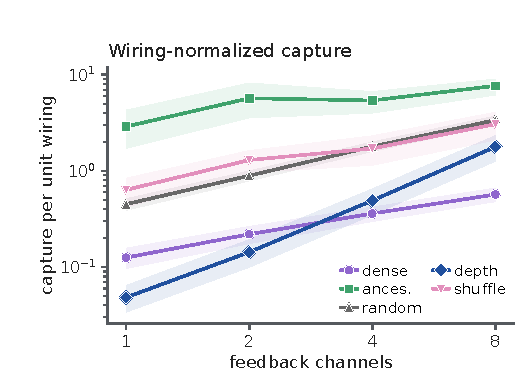
\includegraphics[width=\linewidth,height=3.80cm,keepaspectratio]{pdf_assets/capture_per_wire.pdf}\par
      {\scriptsize\color{Mute}Most of the gain is sparsity; morphology adds a
       bounded anatomy-specific margin.\par}
    \end{column}
  \end{columns}
  \vfill
  \takeaway{Real arbors are economical route dictionaries, but route availability is not evidence of route use.}
  \vspace{0.04cm}
\end{frame}

% 21 — focal shunting with boundary
\begin{frame}{Focal shunting changes descendant transport conditionally}
  \framesubtitle{The established result is transport selectivity, not a generic improvement in trained learning.}
  \begin{columns}[T,onlytextwidth]
    \begin{column}{0.37\textwidth}
      \centering
      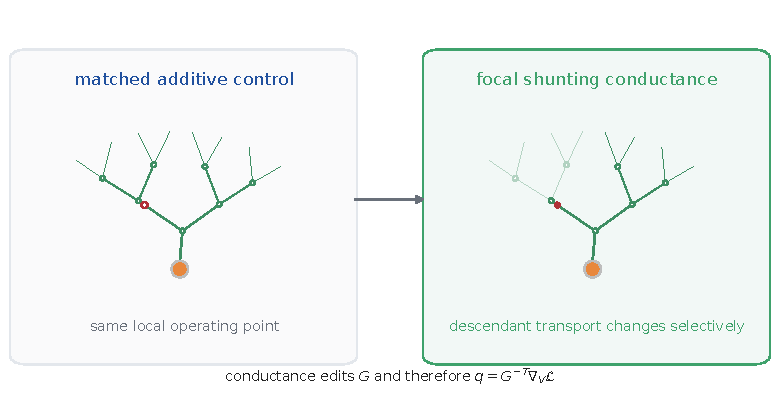
\includegraphics[width=\linewidth,height=2.25cm,keepaspectratio]{pdf_assets/focal_shunt_schematic.pdf}\par
      \vspace{0.06cm}
      \headline[Shunt]{$0.069$}{shunt-minus-additive localization contrast;
        matched local voltage, somatic state, and output error}
    \end{column}
    \begin{column}{0.31\textwidth}
      \centering
      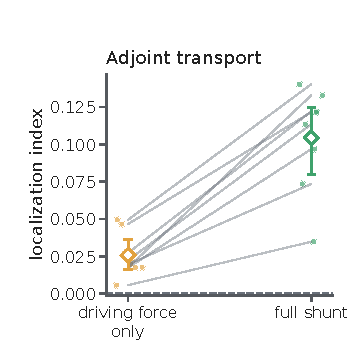
\includegraphics[width=\linewidth,height=3.55cm,keepaspectratio]{pdf_assets/transport_contrast_h.pdf}\par
      {\scriptsize\color{Mute}freezing the adjoint removes the contrast;
       restoring full transport recovers it\par}
    \end{column}
    \begin{column}{0.28\textwidth}
      \centering
      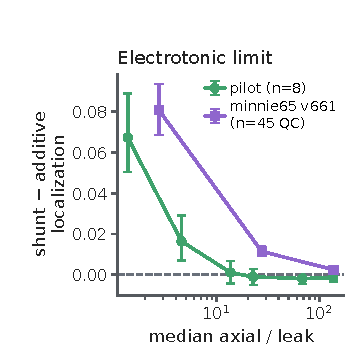
\includegraphics[width=\linewidth,height=3.05cm,keepaspectratio]{pdf_assets/focal_boundary.pdf}\par
      \vspace{0.08cm}
      \claimbox{\tiny Null at textbook resting calibration; present in
        high-conductance regimes. The exploratory adaptive-shunting study did
        not improve final loss over no shunt.\par}
    \end{column}
  \end{columns}
  \vfill
  \takeaway{Conductance can edit route gain locally, but this does not imply an unconditional learning advantage.}
  \vspace{0.04cm}
\end{frame}

% 22 — measured functional null
\begin{frame}{Measured responses show no morphology-specific alignment}
  \framesubtitle{Complete-tree visual-response credit is not better captured by ancestry routes than matched controls.}
  \begin{columns}[T,onlytextwidth]
    \begin{column}{0.30\textwidth}
      \centering
      \CreditTree[mode=address,K=4,scale=0.54,
        stagelabel={same arbor; competing dictionaries}]
      \vspace{0.08cm}
      {\fontsize{17}{19}\selectfont\bfseries\color{Mute}null\par}
      {\fontsize{7.5}{9}\selectfont\color{Mute}ancestry-minus-control
        intervals include zero\par}
    \end{column}
    \begin{column}{0.66\textwidth}
      \centering
      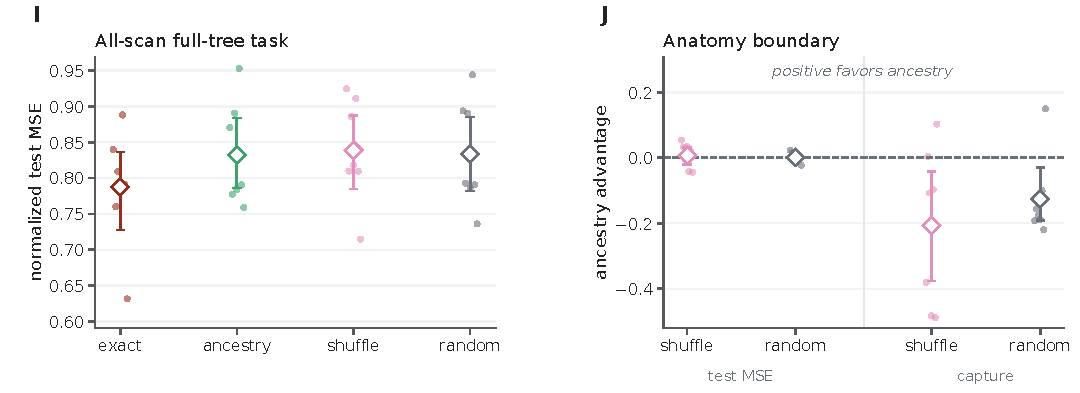
\includegraphics[width=\linewidth,height=4.10cm,keepaspectratio]{pdf_assets/fulltree_no_signed.pdf}\par
      {\scriptsize\color{Mute}Exact fields fit best; ancestry and matched
       low-rank controls remain statistically similar.\par}
    \end{column}
  \end{columns}
  \vfill
  \takeaway{Measured visual responses show no endogenous alignment with ancestry routes.}
  \vspace{0.04cm}
\end{frame}

% 23 — controlled alignment rescue
\begin{frame}{Task alignment rescues the same anatomical dictionary}
  \framesubtitle{Anatomy and channels stay fixed; only the task-gradient direction rotates.}
  \begin{columns}[T,onlytextwidth]
    \begin{column}{0.50\textwidth}
      \heroeq[alignment dose]{%
        \bm g(a)=\sqrt a\,\bm u_{\parallel}
          +\sqrt{1-a}\,\bm u_{\perp},
        \qquad \lVert QQ^{\mathsf T}\bm g(a)\rVert^2=a}
      \vspace{0.10cm}
      \headline[Violet]{$\rho_s=0.99$}{field capture predicts 20-step progress}
      \vspace{0.10cm}
      \claimbox{\footnotesize At $a=0$, nested routes lose to matched controls
        in 8/8 cells; at $a=1$, they win in 8/8.\par}
    \end{column}
    \begin{column}{0.46\textwidth}
      \centering
      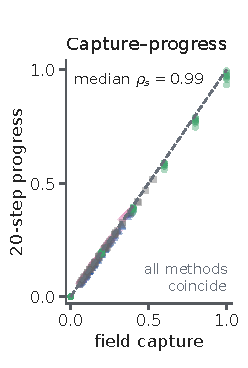
\includegraphics[width=\linewidth,height=4.20cm,keepaspectratio]{pdf_assets/alignment_rescue_n.pdf}\par
      {\scriptsize\color{Mute}Same cells, rank, gradient energy, and curvature;
       only alignment changes.\par}
    \end{column}
  \end{columns}
  \vfill
  \takeaway{Alignment can turn anatomical route capacity into a learning benefit.}
  \vspace{0.04cm}
\end{frame}

% 24 — external animal evidence
\begin{frame}{Animal learning is consistent with signed neuron coordinates}
  \framesubtitle{This is consistent with the first spatial rung; within-tree transport remains unmeasured.}
  \begin{columns}[T,onlytextwidth]
    \begin{column}{0.40\textwidth}
      \centering
      \vspace{0.16cm}
      \begin{tikzpicture}[line cap=round]
        \CTminitree{0}{0}
        \CTminitree{2.05}{0}
        \node[font=\scriptsize\bfseries,text=Shunt,anchor=north] at (0.02,-0.28) {P$^{+}$};
        \node[font=\scriptsize\bfseries,text=BP,anchor=north] at (2.07,-0.28) {P$^{-}$};
        \draw[Shunt,-{Stealth[length=4pt]},line width=1.0pt] (0.95,0.45)--(0.95,1.15);
        \draw[BP,-{Stealth[length=4pt]},line width=1.0pt] (3.00,1.15)--(3.00,0.45);
        \node[font=\tiny,text=Shunt,anchor=south] at (0.95,1.22) {$+$};
        \node[font=\tiny,text=BP,anchor=north] at (3.00,0.38) {$-$};
      \end{tikzpicture}
      \headline[Add]{$83.7\%$}{of contrast energy lies in the signed,
        neuron-specific mode; 6/6 animals}
      {\scriptsize\color{Mute}causal signs were fixed by the BCI mapping and
       predict opposite dendritic contrasts\par}
    \end{column}
    \begin{column}{0.56\textwidth}
      \centering
      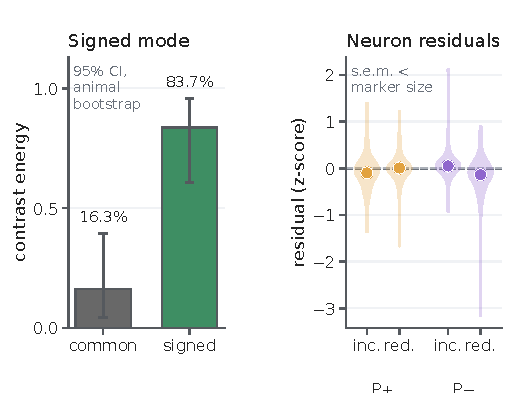
\includegraphics[width=\linewidth,height=4.75cm,keepaspectratio]{pdf_assets/animal_signed.pdf}\par
    \end{column}
  \end{columns}
  \vfill
  \takeaway{The animal result is consistent with signed neuron coordinates; routing within a tree remains open.}
  \vspace{0.04cm}
\end{frame}

% 25 — populated evidence plane
\begin{frame}{One phase plane organizes the positive and null results}
  \framesubtitle{Markers are measured or simulated outcomes; the background is the theory-guided regime map.}
  \centering
  \vspace{0.08cm}
  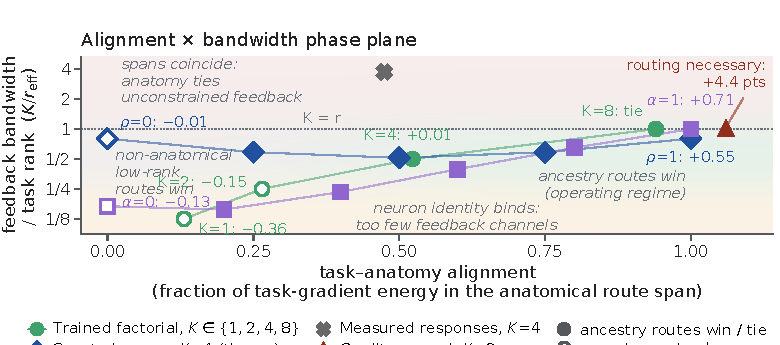
\includegraphics[width=0.96\linewidth,height=5.05cm,keepaspectratio]{pdf_assets/phase_plane.pdf}\par
  \vfill
  \takeaway{The same signal–noise theory explains where dendritic routes help and where they do not.}
  \vspace{0.04cm}
\end{frame}

% 26 — resource ledger, predictions and close
\begin{frame}{Dendrites change the resource ledger, not the exact ceiling}
  \framesubtitle{The contribution is structured local credit routing, conditional on alignment.}
  \begin{columns}[T,onlytextwidth]
    \begin{column}{0.31\textwidth}
      \deftag{exact ceiling}\par
      \vspace{0.08cm}
      {\footnotesize A point system given the same routed field matches the
       dendritic implementation. Exact backpropagation remains the
       first-order ceiling.\par}
      \vspace{0.16cm}
      \centering
      \CreditTree[mode=address,K=4,scale=0.39,
          stagelabel={same routed field}]\par
    \end{column}
    \begin{column}{0.34\textwidth}
      \deftag{what the tree contributes}\par
      \vspace{0.12cm}
      {\footnotesize\good{1.} local conductance state\par}
      \vspace{0.14cm}
      {\footnotesize\good{2.} reusable within-neuron addresses\par}
      \vspace{0.14cm}
      {\footnotesize\good{3.} branch-local route-gain control\par}
      \vspace{0.14cm}
      {\footnotesize\good{4.} sparse feedback wiring\par}
      \vspace{0.26cm}
      \headline[Shunt]{$85\%$ at $7\%$}{dense capture at a small fraction of dense wiring}
    \end{column}
    \begin{column}{0.31\textwidth}
      \deftag{decisive experiments}\par
      \vspace{0.12cm}
      {\footnotesize\textbullet\ focal inhibition should shift plasticity
       below the branch\par}
      \vspace{0.14cm}
      {\footnotesize\textbullet\ the shift should scale with dose and input
       resistance, then saturate\par}
      \vspace{0.14cm}
      {\footnotesize\textbullet\ useful routing should track task–route
       alignment, not morphology alone\par}
      \vspace{0.18cm}
      \centering
      \CreditTree[mode=shunt,shunted=true,scale=0.58,
        stagelabel={focal test of route gain}]
    \end{column}
  \end{columns}
  \vfill
  \takeaway{Coordinates select neurons; trees address synapses; conductance tunes route gain; alignment decides whether any of it pays.}
  \vspace{0.04cm}
\end{frame}
